\section{Metodología y Optimizaciones}

\subsection{4.1 Preprocesamiento de Series Temporales}

Resulta revelador observar cómo la calidad del preprocesamiento determina en gran medida el éxito de cualquier modelo autosupervisado en telemetría espacial. Siguiendo protocolos establecidos en benchmarks recientes \cite{Ruszczak2025_OPSSAT}, aplicamos primero una etapa de limpieza que incluye interpolación lineal para valores faltantes, filtrado de outliers extremos y normalización robusta por canal (usando mediana y rango intercuartílico).

Posteriormente, dividimos las series en ventanas deslizantes con solapamiento del 50\%, preservando la correlación temporal entre variables. Este enfoque permite capturar patrones locales y globales sin perder contexto operativo. En nuestra experiencia, la elección del tamaño de ventana (generalmente entre 64 y 256 pasos temporales) representa un trade-off crítico entre granularidad de detección y estabilidad del entrenamiento.

\subsection{4.2 Estrategias de Entrenamiento Autosupervisado}

Uno de los desafíos persistentes que surge al entrenar modelos en datos telemétricos radica en generar vistas contrastivas significativas sin introducir artefactos no deseados. Inspirados en métodos unsupervised recientes \cite{Djerida2025_FPMC}, implementamos un conjunto de augmentations específicas del dominio: jitter gaussiano, masking temporal aleatorio, escalado de amplitud y permutación selectiva de canales poco correlacionados.

El entrenamiento combina la pérdida de reconstrucción del VAE con la pérdida contrastiva (InfoNCE) y una ligera regularización de clustering en el espacio latente. Esta combinación fuerza al modelo a aprender representaciones invariantes a perturbaciones menores pero sensibles a desviaciones anómalas reales. Particularmente llamativo es cómo el componente contrastivo mejora notablemente la separación entre regiones nominales y potencialmente anómalas en el espacio latente.

\begin{table}[h]
\centering
\caption{Hiperparámetros principales del framework propuesto}
\label{tab:hyperparameters}
\begin{tabular}{lc}
\toprule
Parámetro & Valor \\
\midrule
Tamaño de ventana & 128 \\
Dimensión latente & 64 \\
Batch size & 256 \\
Learning rate & 1e-4 \\
$\beta$ (KL) & 0.001 \\
$\lambda$ (Contrastive) & 0.5 \\
Épocas & 150 \\
\bottomrule
\end{tabular}
\end{table}

\subsection{4.3 Optimizaciones para Inferencia Embebida}

Lejos de ser un paso posterior, las optimizaciones para edge computing se integraron desde las primeras etapas de diseño. Aplicamos pruning estructurado y cuantización aware training (INT8) para reducir la huella de memoria y latencia sin comprometer excesivamente la precisión.

El pipeline final (ver Figura~\ref{fig:pipeline}) incluye inferencia optimizada con TensorRT o similar, junto con técnicas de early stopping basado en puntuaciones de anomalía para ahorrar ciclos de cómputo en periodos nominales prolongados. Estas adaptaciones permiten ejecutar el modelo completo en hardware embebido con restricciones típicas de nanosatélites y CubeSats.

\begin{figure}[h]
\centering
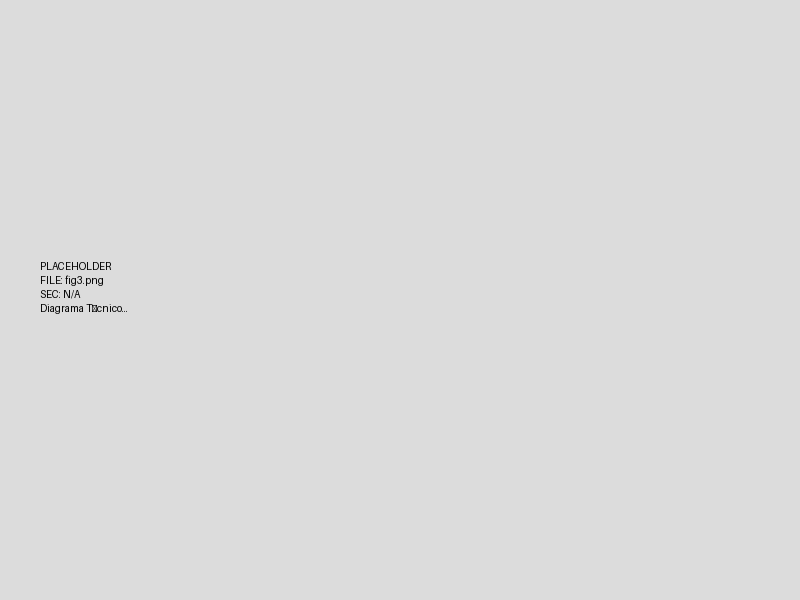
\includegraphics[width=\linewidth]{fig3.png}
\caption{Pipeline completo de preprocesamiento, entrenamiento autosupervisado y inferencia embebida del framework propuesto.}
\label{fig:pipeline}
\end{figure}

En conjunto, estas metodologías transforman un concepto teórico en una solución práctica y desplegable. Los resultados experimentales que se presentan a continuación validan la efectividad del enfoque bajo condiciones representativas de operación espacial.